\documentclass[a4paper,12pt]{article}
\usepackage{ecography}
\usepackage{lmodern}
\usepackage{amsmath}
\usepackage{xfrac}
\usepackage{lineno}



 \renewcommand{\familydefault}{\sfdefault}

\nolinenumbers

\title{A Recipe for Scavenging - the natural history of a behaviour}
%TG: nice title! I'd replace the hyphen with a comma though
\running{Scavenging in vertebrates}

\author{Adam Kane, Kevin Healy, Thomas Guillerme, Graeme Ruxton, \& Andrew Jackson.}

\affiliations{
\item A. Kane (\url{adam.kane@ucc.ie}), University College Cork, Cooperage Building, School of Biological Earth and Environmental Sciences, Cork, Ireland.
\item K. Healy and A.L. Jackson, Trinity College Dublin, Department of Zoology, School of Natural Sciences, Dublin 2, Ireland; Trinity Centre for Biodiversity Research, Trinity College Dublin, Dublin 2, Ireland.
\item T. Guillerme, Imperial College London, Silwood Park Campus, Department of Life Sciences, Buckhurst Road, Ascot SL5 7PY, United Kingdom.
\item G. Ruxton, School of Biology, Sir Harold Mitchell Building, Greenside Place, St Andrews, KY16 9TH, United Kingdom.
}

\nwords{9999}


\begin{document}

\maketitle


\begin{abstract} 
Despite its prevalence, scavenging is a difficult behaviour to observe in modern day carnivores and impossible to study directly in extinct species. 
Yet, there are certain intrinsic and environmental features of a species that push it towards a scavenging lifestyle. 
These can be thought of as some of the principal parameters in optimal foraging theory namely, encounter rate, handling time and prey availability. 
We use these components to highlight the morphologies and environments that would have been conducive to scavenging over geological time by focusing on the dominant vertebrate groups of the land, sea and air. 
The result is a synthesis on the natural history of scavenging, the first to our knowledge. 
Our idea of a scale of scavenging can be applied to any species at any time to judge the importance of this behaviour in its diet. 
\end{abstract}

\newpage


\section*{Introduction}


Historically, scavengers have not been viewed as the most charismatic of animals.
This may go some way to explaining the gap in our knowledge of the prevalence of this behaviour \citep{devault2003scavenging}.
Professor Sanborn Tenney writing in 1877 for The American Naturalist had this to say about one well known group, ``prominent among the mammalian scavengers are the hyenas, the ugliest in their general appearance of all the flesh eaters."
He contrasts these with ``nobler kinds" of carnivores such as lions and tigers \citep{tenney1877few}.
Even aside from our own subjective biases, scavenging is a difficult behaviour to detect after the fact.
Without catching a carnivore in the act of killing we are left to infer how the prey was killed.
Some simple heuristics can inform us, for instance, in cases where the prey item was simply too large to have been killed by the ostensible predator \citep{pobiner2008paleoecological}.
But clearly, a scavenger does not only feed on animals too big for it to have hunted.
The obvious lack of direct behavioural data compounds the difficulty of discerning scavenging from predation among extinct forms.
Indeed, a single species of dinosaur notwithstanding \citep{carbone2011intra}, a synthesis describing the natural history of scavengers is absent from the literature.
With research on scavenging on the rise \citep{manga2006vulture} we are now beginning to realise the extent of this behaviour such that, ``in some ecosystems, vertebrates have been documented to assimilate as much as 90\% of the available carrion" \citep{beasley2015vertebrates}.
This has profound implications for the trophic ecology of these systems and particularly our models of them.
Even Tenney’s noble big cats are now known to take in a significant portion of carrion in their diet where some lion populations acquire over 50\% of their meat from carcasses \citep{jones2015african}.
While recognising the difficulty in directly observing scavenging, it is possible to turn to other methods in order to discern the most suitable morphologies, physiologies and environments for a scavenging lifestyle to prosper.
Here we chart the natural history of scavenging by assessing the potential for the behaviour in dominant vertebrate groups given their ecology and functional traits.
%It is our aim in this review to employ these methods to gain an understanding of scavengers past and present.

%the intro needs to lead towards a aim a bit more strongly

\subsection*{The Challenges of Scavenging} 
The chief hurdle to scavenging is finding a resource that is often difficult to predict in space and time.
Through chance alone many species will avail of some opportunistic scavenging. 
However, species that rely on scavenging to sustain substantial portions of their diets must encounter a sufficient amount of carrion in order to meet their energetic demands.
Once found, the scavenger must be able to out-compete any potential competitors and efficiently process the, typically decaying, carcass replete with micro-organism derived toxins  \citep{ruxton2014fruit}. 
These characteristics can be assumed to be under evolutionary selection pressures for traits that increase carrion discovery and monopoly.
Finally, the potential for scavenging will also depend on the density, size, and quality of carcases produced, all of which are affected by complex ecosystem dynamics but are outside the selection pressures on the scavenger.
Each of these facets are essentially the backbone of fundamental ecological theory and are the key parameters defined in functional response curves, namely encounter rate, handling time and prey availability \citep{jeschke2002predator}.  
By considering scavenging in this context of optimal foraging we can identify the prerequisite attributes and processes required for the behaviour. 
This has enabled us to propose a scale of scavenging whereupon we can place any vertebrate species, past or present, and assess the likely importance of carrion in its diet. 

\begin{figure}[!htbp]
\centering
   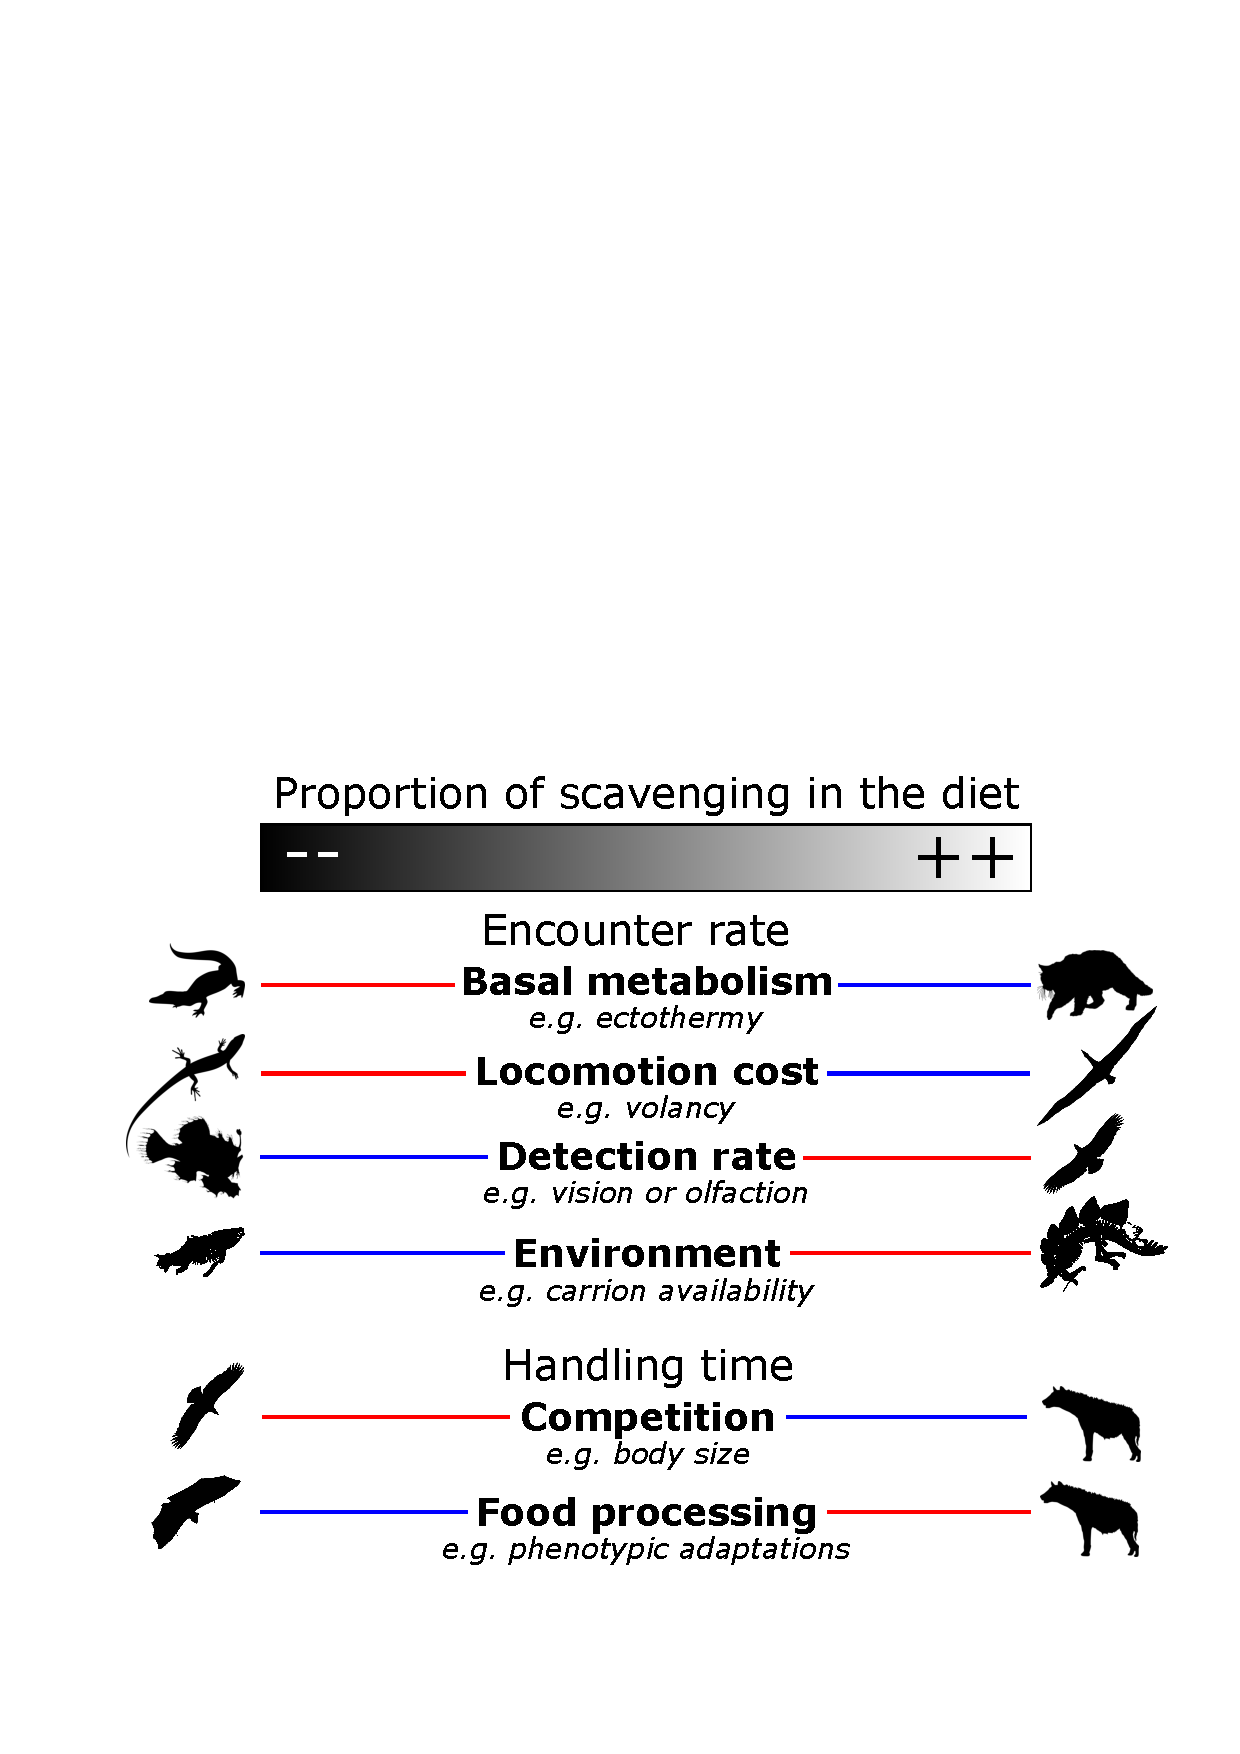
\includegraphics[width=1\textwidth]{Summary_figure/Summary_figure.pdf}
\caption{Factors influencing the proportion of scavenging in a vertebrates' diet. The black and white gradient bar on the top represent the proportion of scavenging in the diet, ranging from low (- -) on the left hand side to high (+ +) on the right hand side. Blue lines indicate that a reduction in the factor will lead to more or less proportion of scavenging in the diet and red lines indicate an increase.}
%Silhouettes from left to right on each line: \textit{Somelizard ofsomesort}, \textit{Felis silvestris}, \textit{Somelizard ofsomesort}, Diomedeidae, \textit{Antennarius striatus}, \textit{Gyps}, Actinopterigii skeleton, \textit{Stegosaurus} skeleton, \textit{Gyps}, \textit{Crocuta crocuta}, \textit{Rousettus aegyptiacus}, \textit{Crocuta crocuta}.
\label{Summary_figure}
\end{figure}


%KH: need paragraph for how do we know something is (was) a scavenger
\section*{Encounter Rate}
All foraging processes depend on the encounter rate between consumer and resource. 
<<<<<<< HEAD
Locomotory speed, foraging time and detection radius all determine the encounter rate between a scavenger and the carcasses it is searching for. 
Alternatively, a species can reduce its metabolic requirements so that it can survive long periods between meals. 
We would thus expect selection pressures to act on the various traits that govern these parameters.  

However, as we noted above, encounter rate is also determined by the productivity of the environment, something which the selective forces acting on the scavenging have no control over. 
=======
Locomotory speed, foraging time and detection radius all determine the encounter rate between a scavenger and the carcasses it is searching for and we would thus 
expect selection pressures to act on the various traits that govern these parameters.
Alternatively, selection might drive a species to reduce its metabolic requirements so that it can survive long periods between meals, or expand a species ability to 
process tissues or decaying flesh that might ordinarily be discarded.  However, as we noted above, 
encounter rate is also determined by the productivity of the environment, and ultimately the rate at which carcasses are produced, 
an aspect which the selective forces acting on the scavenger have no influence. 
>>>>>>> origin/master

%As such, scavenging potential is strongly affected by search rates, which are determined by anatomy, physiology and behaviour which are all under selective pressure, as well as the type of environment the scavenger is foraging in.

\subsection*{Metabolism}
Because of the sporadic nature of carrion we would expect adaptations that reduce energetic costs of maintenance to be selected for in scavengers as it would allow for longer inter-feeding periods. 
Extant reptiles possess an advantage here, in that over the course of a year their food requirements can be 30 times lower than an endotherm of equal size \citep{Nagy1621}.
\cite{devault2002scavenging} suggest this is an avenue for scavenging in snakes because they ``exhibit exceedingly low maintenance metabolisms, and most can survive on a few scant feedings per year.
It is, therefore, possible for snakes to rely largely on infrequent, less energy-rich meals."
In the same review the authors found occurrences of scavenging spread across five families of snakes and stated that this behaviour is ``far more common than currently acknowledged."\citep{devault2002scavenging}.
The same reasoning can be applied to crocodiles and their allies \citep{forrest2003evidence,moleon2015carcass}. 
\cite{carey1982temperature} found ectothermic sharks have the ability to go weeks between meals because they focus on the energy-rich sections of carcasses (see Handling Time). 
Endotherms have also evolved physiological mechanisms that allow them to depress their otherwise high metabolic rates at certain times e.g. vultures who do so while resting at their roost and during periods of food deprivation \citep{bahat1998nocturnal}. 

\subsection*{Locomotion}
The inherent unpredictability of carrion also means scavenging depends more on the ability to efficiently move over larger areas than does predation.
This generally requires an efficient transfer of metabolic energy into movement which relies on the animal's anatomy and physiology as well as the medium of the environment in which the animal is moving (i.e. aerial, aquatic or terrestrial).
Perhaps the most efficient form of locomotion in vertebrates is, paradoxically, found in flying species. 
Despite the energetic costs of flight, the only known vertebrate obligate scavengers are the old and the new world vultures. 
While powered flight is energetically expensive, species like vultures have evolved behavioural and anatomical features to exploit air currents using their large wingspans, allowing them to soar at a cost of only twice their metabolic rate \citep{hedenstrom1993migration,spivey2014analysing}.
By depending on thermal air flows these species can forage over vast ranges \citep{spiegel2013factors}. 
An analogous mode of locomotion is also exploited by seabirds, who use strong ocean winds to search large areas of the oceans \citep{norberg2012vertebrate,thaxter2012seabird}. 
While many species of seabird are likely primarily predators, it seems that albatrosses, who can range many hundreds of kilometres, take a substantial amount of carrion in their diet \citep{croxall1994dead}. 
This is typically in the form of squid carcases, which float on the surface, allowing the birds to readily pluck their remains out of the water \citep{croxall1994dead}. 

The groups from which these modern soaring birds arose, appear during the Palaeocene \citep[66 - 56 Million years ago (Mya); ][]{Jetz2012, Jarvis2014} and Cretaceous \citep{chiappe2006early} respectively. 
However, soaring flight is likely to be far older than this with avian flight originating in the Late Jurassic (163.5-145 Mya) and vertebrate flight in the Late Triassic (235-201.3 Mya) coincident with the pterosaurs. 
Indeed, scavenging among pterosaurs has been hypothesised many times before \citep{witton2008reappraisal}. 
Certain groups of these animals could reach enormous sizes \citep[e.g. Azhdarchids with wingspans of 11 metres; ][]{witton2010size} and, notably, appear to have engaged in soaring flight \citep{witton2010size}.
It seems probable that at least some of these extinct species used soaring as a means for scavenging \citep{witton2013pterosaurs}. 
%KH added "at least some of these" as it was not clear what species used soaring as a means for scavenging.
While soaring is perhaps the only viable means of locomotion that allows for an obligate, scavenging life-style \citep{ruxton2004obligate}, powered flight is still an efficient means of locomotion. 
Certainly, avian flight is cheaper than either walking or running \citep{tucker1975energetic}.

We know that many extant birds exist as facultative scavengers because storks, raptors and corvids all take substantial quantities of carrion in their diet \citep{kendall2013alternative}. 
Similarly we would expect that extinct species would also scavenge in a similar fashion depending on the efficiency of their flight. 
For example, early birds such as \textit{Archaeopteryx} are predicted to have been poor, relatively inefficient fliers \citep{nudds2010narrow} and so ill-suited to finding carrion. 
The importance of efficient flying over large areas may explain the lack of scavenging behaviour in bats as they are generally nocturnal, a time when they would receive no aid from convective air currents \citep{norberg2012vertebrate}. 

Similar to aerial species, aquatic scavengers have a locomotory benefit because water is a medium that is conducive to low-cost movement \citep{tucker1975energetic,williams1999evolution}.
This has led some researchers to argue for the likelihood of an obligate scavenging fish \citep{ruxton2004energetic,ruxton2005searching}. 

Sharks are one likely candidate for general scavenging behaviors as their locomotion, which depends on large pectoral fins to generate lift as they swim, resembles that of the large soaring fliers.
Many shark species have large foraging ranges \citep[e.g. the great white sharks \textit{Carcharodon carcharias};][]{bruce2006movements} and it seems reasonable that they would use oceanographic currents to further reduce movement costs \citep{ruxton2004energetic}.
In fact, facultative scavenging is seen in many selachian groups, including species of extant sharks like white sharks \citep[known to feed on whale carcasses;][]{fallows2013white}, Greenland sharks \citep[feeding on seals;][]{watanabe2012slowest}, and sixgill sharks \citep{anderson2016impact}. 
There is evidence too of scavenging in extinct species, where shark teeth have been found in the remains of dinosaurs, mosasaurs and Pliocene mysticete whales \citep[5.3-3.6 Mya; ][]{schwimmer1997scavenging,ehret2009caught}. 

Interestingly, style of swimming in fish does not significantly affect the cost of movement \citep{williams1999evolution}, hence it is likely that many aquatic species with large ranges will encounter scavenging opportunities. 
It is perhaps jaw morphology that is more likely to define which species can avail of carcasses.
%KH I moved this down here as it kinda throws our shark soaring thing out the window (which I like as a linking function). However I think this kinda solves our problems in the complexity of swimming by saying apart from large ranges ability to eat is probably more important.

We might expect then that by combining an aquatic environment and an endothermic metabolism marine mammals would especially prosper as scavengers. %, especially as this group has perhaps the largest home range of any animals (whales and shit).
Fossil pinnipeds and cetaceans from 60 Mya have transitional features indicative of their evolutionary trajectory to fully aquatic species \citep{williams1999evolution}.  
But despite their movement away from land their energetic savings were negligible because the \textit{total} cost incurred by a swimming marine mammal is high \citep{williams1999evolution}. 
Indeed, the total energetic cost is similar to an equivalent terrestrial or aerial mammal \citep{williams1999evolution}.
This underscores the trade offs between the benefits of endothermy in terms of activity periods and the costs of maintaining such an energetically expensive system. 
That said, aquatic endotherms have and do scavenge. 
For instance, early whales such as \textit{Basilosaurus} (38-36.5 Mya) seem to have fit into the same niche as killer whales (\textit{Orcinus orca}) and we have some evidence for scavenging in both \citep{fahlke2012bite,Whitehead415}.

%%KH Is there anything we should add about other extinct groups such as plesiosaurs and https://en.wikipedia.org/wiki/Plesiosauria#Gait maybe an air breathing non-airbreathing devide would be good.


%% AK:  Need to be careful here because this whole idea of sprawling posture being worse off than erect posture is not that well supported in the literature. 
%% Great Transformations in Vertebrate Evolution By Kenneth P. Dial, Neil Shubin, Elizabeth L. Brainerd talks about it at length 
%% So I think this should stay pitched as an endo/ ectothermy thing rather than posture 
Terrestrial environments are the most energetically costly in which to move \citep{tucker1975energetic}. 
Unlike aerial and aquatic environments support must be provided through the animal's posture. % leading to trade offs between low cost of maintain and the efficiency of transport. 
The early transition from a sprawling gait, seen in early tetrapods, to the more erect posture of synapsids and later dinosaurs and mammals, has often been supposed as conferring a huge advantage to the latter groups \citep{sullivan2015posture}.
The purported advantages include benefits in terms of speed, efficiency, muscle effort and manoeuvrability \citep{sullivan2015posture}.
Clearly, for a scavenger, an ability to efficiently cover an area at a high speed would increase the encounter rate with carrion. 
Despite being intuitive, \cite{sullivan2015posture} states most of the hypotheses in favour of this idea remain to be tested in the context of archosaur evolution. 
One noted consequence of a sprawling gait is the phenomenon known as Carrier's constraint such that the animal can't move and undergo costal ventilation at the same time because the lateral movements impedes its lungs \citep{carrier1987evolution}. 
The evolution of an upright posture has been offered as one of the primary mechanisms that allowed early archosaurs to overcome this constraint \citep{uriona2008recruitment}. 


% For example, the sprawling posture of many ectotherm groups (except frogs!) would be expected to allow for a lower maintenance cost relating to body support in comparison to groups with the limbs position underneath the body, such as mammals, aves and dinosaurs.
%KH: I agree with TG and have removed the gas exchange thing as its a physiology thing only applicable to certain groups and not got to do with terrestrial environments really. I also removed the 
%Also that reference is from 1975, is this up to date?

% While the low maintenance costs of a sprawling-like posture may reduce the need to scavenge frequently, the ability to search large areas quickly is severely restricted in these groups reducing scavenging opportunities (ref on home range of terrestrial ectoterms). 
% For example, a sprawling gait results in 
% On the other hand the more erect body positions and often associated higher basal metabolic rates, allow for sustained locomotion over long periods of time allowing such species to search large areas.



%KH Even after changing it I dont like this transition type narrative.
%KH also needs to be more clear on what the advantage to scavenging is for these groups.
%
%none of these advantages refer very clearly to scavenging
%KH I'm always wary of deeming something as intuitive, 

%Metabolic rate however, unquestionably impacts terrestrial species whereby ectotherms such as many modern reptiles, cannot move for sustained periods \citep{bennett1979endothermy}. 
% Species which do not support an upright position such as modern reptiles limit their ability to move for sustained periods \citep{bennett1979endothermy}. 

%KH I think as ectothermy is almost completely associated with sprawling gaits I would tie it up together to avoid repeating something similar here.

%This is exacerbated by their sprawling gait which results in the phenomenon known as Carrier's constraint such that the animal can't move and breathe at the same time because the lateral movements impedes its lungs \citep{carrier1987evolution}. 
% These constraints are likely to mean that many ectotermic terrestrial species, which cannot maintain an upright posture would depend on a relatively low level of scavenging (I'm not sure this is true though). 
%This would also have been true of extinct species with the same physiology. 
%TG: I guess this is a comment too: Snakes are a bit different are more effecent at moving I think - lots of scavanging. 
%Both these groups are more likely to depend on low energetic costs in order to compensate for low encounter rates due to their inability to move. 
 
% Although the earliest evidence of vertebrate scavenging comes from the Permian (298.9 - 252.17 Mya) where a temnospondyl amphibian fed on the carcass of \textit{Varanops}, a predatory synapsid of the time \citep{reisz2006articulated}. 
Whatever the case, it is with the evolution of endothermy in the therapsid-mammal lineage \citep{clarke2010temperature} that terrestrial vertebrates would have gained the ability to range more widely, a vital component in seeking out carrion.
Modern endothermic mammals can sustain longer periods of energetically expensive activity \citep{bennett1979endothermy} resulting in larger foraging ranges. 
Today, terrestrial scavenging in the mammals is probably best known in an African context where hyenas, jackals and lions all take sizeable proportions of carrion in their diet.
In the spotted hyena (\textit{Crocuta crocuta}), striped hyena (\textit{Hyaena hyaena}) and brown hyena (\textit{Hyaena brunnea}) it can be over 90\% \citep{jones2015african}.
And although no contemporary terrestrial vertebrate exists as an obligate scavenger, most, if not all, are facultative to some extent \citep{beasley2015vertebrates}.
The particular reliance of hyenas on carrion means we can use them as examples of efficient terrestrial scavengers to compare with other forms. 
In terms of locomotion, they employ a characteristic ``rocking horse gait"  which allows them to cover great distances efficiently, loping at 10 km/hr \citep{mills1989comparative,jones2015african}. 
Such long-distance travel is apparent in African wild dogs (\textit{Lycaon pictus}) and many other canids \citep{pennycuick1995radius,janis2014forelimb}. 
In contrast, big cats like leopards (\textit{Panthera pardus}) rely on ambush \citep{pennycuick1995radius}. 
This allows us to make a broad distinction between the ambush strategies of cat-like forms and the pursuit/ pounce strategies of more dog-like forms, the latter being more suited to scavenging \citep{janis2014forelimb}. 
These insights allow us to compare extant terrestrial species to their prehistoric forebears given the dominance of mammalian carnviores since the Eocene (56-33.9 Mya) where the order split into the Caniforma and Feliforma \citep{van1987skeletal}.
To take one example, \cite{anyonge1996locomotor} found that \textit{Nimravides}, a genus of sabretooth cat from the Miocence (10.3 to 5.3 Mya), were likely to have been ambush predators which would argue against them taking a lot of carrion. 


Of course, terrestrial animals can also move bipedally. 
Although the evolution of bipedal  movement was significant in that it freed up the forelimbs for other purposes (e.g. climbing, tool-use, wing development etc.) it does not differ radically in cost from quadrupedal locomotion (\cite{williams1999evolution}, and references therein). 
For instance, \cite{alexander2004bipedal} shows  that, in the case of humans, we are more economical than predicted while walking and less so while running according to predicted costs of terrestrial movement calculated by allometric scaling relationships.
Our locomotory efficiency has fed into the question of where our ancestors placed on the hunter-scavenger axis during the Plio-Pleistocene, which has been a matter of debate for years \citep{dominguez2002hunting}.
\cite{ruxton2013endurance} added to this debate with their argument that long distance endurance running, often used by humans for hunting, was not an important feature of hominin scavenging.
They arrive at this conclusion on the basis of the high cost of running coupled with the fact that dangerous competitors will tend to arrive beforehand. 


% While we can use modern analogues of quadrupedal species, the lack of scavenging in bipeds makes this more difficult. However, bipedal locomotion may have been a particularly useful strategy for searching large areas. For instance, \cite{alexander2004bipedal} shows that, in the case of humans, we are more economical than predicted while walking according to predicted costs of terrestrial movement. In fact the ability of humans to engage in hunting strategies that involve traversing long distances, such as persistence hunting, has led to several researches highlighting the possible role of scavenging in early hominids. Indeed the low energetics of human walking at least allows for a substantial amount of scavenging in our hominid ancestors (Graemes papers on scavenging).
%%KH I know this is excluding other hominids so feel free to write a more inclusive line.

Aside from humans and our allies, the best-known terrestrial bipeds are the dinosaurs and unsurprisingly, given their enduring appeal, the prevalence of scavenging has been extensively explored in the carnivorous theropods.
These were the dominant terrestrial carnivores for most of the Mesozoic Era (252.17 - 66 Mya) and ranged from the chicken-sized to the whale-sized, all of which were bipedal.
While the locomotory ability of theropods has been debated since their first inception, more recent studies have reconstructed them as relatively mobile animals \citep{pontzer2009biomechanics}. 
Despite some suggestions that larger species may have had some advantage in scavenging, partially due to the ability to search large areas \citep{ruxton2003could}, more recent work has shown that the energetic demands of such large forms meant scavenging was likely more prevalent in mid-sized theropods of approximately half a tonne \citep{kane2016body}.

%They are quite alien to anything we know today which restricts our ability to understand their ecology far more so than extinct mammals \citep{weishampel2004dinosauria}.
%Of relevance, are the questions that still persist about their metabolism, with the latest evidence suggesting they were mesothermic \citep[i.e. intermediate to ecto- and endotherms;][]{grady2014evidence}.
%KH Do we need to get into this?
%We do know that they walked with the erect gait of mammals or birds rather than the sprawling gait of lizards and that they were most likely facultative scavengers \citep{weishampel2004dinosauria,depalma2013physical}.
%KH Is this not a bit trivial almost?
%Taken together, this implies dinosaurs had a foraging range that fell in between that of modern terrestrial mammals and reptiles. 
%I don't think we can say that, we have no idea on thier range. For example using body size they should be larger than modern mammals, however the importance of metabolic rate is still not clear with home range (body size explains most.). This might be useful http://www.jstor.org/stable/10.1086/682070?seq=1#page_scan_tab_contents

%KH I think the terrestrial section needs a little more work still, it doesn't hang together quite right yet although it is not far off it. While I have wrote it up this way I think ending with humans would be good as it gives a returning to the present type feel which wraps the whole section up without being too explicit about it. Maybe using large bird locomotion would allow this.



\subsection*{Detection}

%KH Just my opinion but I found it really difficult to understand the flow of this section. I starts off with a type of 2d- 3d thing but then kinda bounces around different ideas with everything talked about in relation to aerial viewing. Its also missing how understanding detection ranges can help us understand past scavenging behavior. I would include in the terrestrial section, the use of looking at the portion of the brain attributed to olfactory sensing (like the way we did the scaling of detection range in our paper) as a possible indicator of scavenging. I would also throw into the social communication section that these behaviors can show how groups can be good scavengers through active/passive communication and we might expect that in other extinct social groups (the vulture thing was almost impossible for pterodactyls to avoid I would say and probably common in many soaring flying species). Also Graeme has a paper on human scavenging about how hominies may have exploited vultures and also probably searched in a social sense. 
%I might be too grumpy at the end of the day, but I think a bit of a restructure might help this section.

As predicted by the importance of an increased encounter rate, known scavengers have evolved well-developed senses, with the visual and olfactory sensory systems most often associated with scavenging behavior. 
This is perhaps no surprise because sensory systems that rely on detecting signals associated with living animals, such as audioception, electroreception, thermoreception and echolocation will be limited in their ability to detect an already dead animal.

Apart from the basic capacity of these senses to detect carrion, how they function in different environments is also important. 
In the simplest case, the search space is a two dimensional plane \citep{pawar2012dimensionality}. 
If the scavenger itself is searching on the plane, as is so for terrestrial species, the detection range is simply defined by the radius of their sensory organs.
Consequently, the ability to detect carrion can be seriously restricted for visually reliant, terrestrial species. 
They may overcome this restriction however, by using olfaction, which is less affected by the relief of the land.
For example, hyenas have the ability to smell a rotting carcass 4 km away \citep{mills1989comparative}, which exceeds the 500 m range deemed necessary by \cite{ruxton2004obligate} to be able to survive as a scavenger. 

Indeed, the olfactory senses of many extant (and in all probability extinct) carnivores meet this required distance, making scavenging feasible for most terrestrial carnivores \citep{farlow1994speculations,mech2010wolves}. 
Among extinct species in particular, we can use the ratio of olfactory bulb to brain size to infer a preference for olfactory foraging \citep{zelenitsky2011evolution}.
This approach was used by \cite{zelenitsky2011evolution} to hypothesise such a mode for the theropod dinosaur \textit{Bambiraptor} and by \cite{witmer2009new} for tyrannosaurs.
The flying pterosaurs however, had tiny olfactory bulbs indicating this sense was not relied on \citep{witton2013pterosaurs}.

Species capable of flight have added an extra spatial dimension (i.e. the vertical component) to their sensory environment over land animals.
This allows them to look down on a landscape where they are unencumbered by obstacles that would obstruct the view of a terrestrial scavenger.
In this way they are effectively cheating the 2D system by gaining a bird's eye view which has has obvious benefits in detecting carrion.
Certainly, vultures are known to have impressive visual acuity, with one estimate indicating lappet-faced vultures (\textit{Torgos tracheliotus}) are capable of detecting a 2 metre carcass over 10 km away \citep{spiegel2013factors}.
Eagles too are known to have highly developed vision \citep{reymond1985spatial}.
The flying pterosaurs also convergently evolved large orbits and optic lobes \citep{witton2013pterosaurs}. 
It follows that the evolution of flight allowed aerial animals to detect far more carrion than their terrestrial counterparts through vision \citep{AR:AR22815}.

Existing in this environment also means being able to gather a wealth of information from other foragers, be they conspecifics or otherwise \citep{jackson2008effect}.
These interactions are properly three dimensional in the sense of \cite{pawar2012dimensionality} because both producer and scrounger are in the air \citep{dall2005information}. 
Again, returning to vultures, the genus \textit{Gyps} consists of highly social and colonially nesting species \citep{fernandez2015density}.
These behaviours allow them to forage far more efficiently because one bird can scrounge information on the location of food from another successful forager \citep{KaneVul}.
Information transfer of this kind is typically inadvertent and as a consequence no complex social interactions are required, simply the ability to recognise a successful forager.
Thus, it seems probable that scrounging behaviours were seen in the flying pterosaurs as well. 

The terrestrial-olfaction, aerial-visual divide is not total though.
Terrestrial species like hyenas and hominins exploit the efficiency of birds by looking to the skies for groups of vultures to follow to carrion \citep{jones2015african,ruxton2013endurance}. 
And many birds, e.g. turkey vultures (\textit{Cathartes aura}), have well-developed olfactory systems \citep{AR:AR22815} which they use to forage in heavily forested areas where vision is limited \citep{houston1986olfaction}. 

Although aquatic species also have a vertical component to their environment, they must contend with low-light levels where visual detection distances are far lower ($<$ 100 m) than they would be for air.
As such, aquatic animals detect resources through chemo- and mechanoreception more so than through vision \citep{ruxton2004energetic}.
This is particularly relevant to sharks and aquatic snakes who are deemed as having the most suitable physiology for scavenging.
A hypothesis put forth by \cite{sazima1990necrofagia} argued that chemical gradients in water would allow for a relatively easier detection of carrion by snakes.
This gained some support from \cite{devault2002scavenging}, who found a preponderance of aquatic snake species in their review of this behaviour.
Smell seems to be the primary means of carcass detection in sharks as well. 
\cite{fallows2013white} found that wind speed determined the number of sharks feeding at whale carcasses, indicating they were dependent on detecting the odours from the decaying whales. 

\subsection*{Prey Availability}
The environmental influence on prey availability is an aspect that greatly affects encounter rate but is invisible to the selective forces acting on the scavenger. 
Aspects including, primary productivity, relief, and temperature will all greatly affect scavenging tendency. 
\cite{ruxton2004obligate} suggest an historic ecosystem with a productivity similar to the Serengeti could have supported an \textit{obligate} mammalian or reptilian terrestrial scavenger.
Indeed, in systems that were dominated by large ectothermic or mesothermic herbivore vertebrates, the same primary productivity would have supported a greater biomass, due to the scaling of mass with metabolic rate \citep{mcnab2009resources}.
The upshot of this may have been a higher biomass of herbivores dying and offering scavenging opportunities (although these larger species may have also lived longer).

In fact, scavenging behaviour may have evolved on land as soon as the first terrestrial tetrapods emerged.
Some of the earlier tetrapods tracks dating back to the early Middle Devonian (393.3 - 387.7 Mya) were found in intertidal environments \citep{Niedzwiedzki2009}.
These environments are isolated from marine systems twice a day leaving potential carrion unexploited by marine vertebrates.
\cite{Niedzwiedzki2009} suggest that these environments ``would thus have allowed marine ancestors of tetrapods gradually to acquire terrestrial competence while accessing a new and essentially untouched resource.''

Staying in the aquatic setting, the phenomenon of occasional bounties of carrion in the form of whale falls has led some researchers to investigate if an obligate scavenger could survive by seeking out these remains exclusively.
\cite{ruxton2005searching} argued that although this is energetically feasible it's ecologically unlikely.
Any animal that could find such whale carcasses is unlikely to have ignored other types of carrion.
Although no aquatic species have ever exceeded the size of whales, some enormous animals have evolved in this environment before the evolution of cetaceans, including \textit{Leedsichthys}, a bony fish from the Middle Jurassic (174.1-163.5 Mya) and the aquatic Mesozoic reptiles, the plesiosaurs, pliosaurs and ichtyosaurs, that could all exceed 15 metres in length \citep{ruxton2011zoology,danise2014ecological}.

So, despite being unlikely, the energetic feasibility of a marine scavenger that specialises on large carcasses has a long history.
One point of interest is that of the whaling industry, which provided a bonanza of floating carcasses especially during the 20th century \citep{Whitehead415}.
This meant killer whales could switch from hunting to scavenging, a switch made that much easier by the noise of the whaling vessels that would effectively ring the ``dinner-bells" \citep{Whitehead415}.

Perhaps the greatest environmental driver of scavenging tendency is that of temperature. 
The geological record shows the Earth has undergone radical fluctuations in temperature over time.
This will have had a significant bearing on the availability and persistence of carrion.
To illustrate the point, a 10$^{\circ}$C increase in ambient temperature can double carcass decomposition rates \citep{parmenter2009carrion} and geological evidence indicates that the Mesozoic Earth was on average at least 6 $^{\circ}$C warmer than now \citep{sellwood2006mesozoic}.
In terms of specific habitats, it has been shown that decomposition is greater in warm and moist areas versus more xeric ones \citep{beasley2015vertebrates}.
Moreover, oceanic productivity and habitat structure are all impacted by climactic conditions.
The impacts these can have on scavengers have been empirically supported e.g. \cite{beasley2015vertebrates} who point to a series of studies showing how microbes and invertebrates benefit at higher temperatures to the detriment of vertebrate scavengers such that ``above 20$^{\circ}$C vertebrates were able to detect and consume only 19\% of small-mammal carcasses, whereas at temperatures below 18$^{\circ}$C, vertebrates consumed 49\% of carcasses".


%Predators were large-bodied too compared to extant mammalian predators \citep{mcnab2009resources}, and so, especially if they were ectothermic, could last longer between meals, rendering scavenging a more attractive behaviour relative to predation.
%%KH Not sure this sentence belongs here, already covered int he handling section.


%Frequently, the interplay between abiotic and biotic factors can impact the ability of an animal to scavenge. 
%We know vultures and eagles tend to soar using thermals and if these air pockets don't form, say on a cloudy day, the bird is grounded \citep{mundy1992vultures}.
%In many habitats (e.g. the Arctic) it is simply not possible for sufficiently powerful thermals to form and as a consequence large-bodied vultures cannot exist.
%% KH I dont think this belong in this section, we probably have covered this enough in the locomotion part.
%One result of this is that t.
%Certainly, a major difficulty for terrestrial scavengers is competition with vultures.
%Nocturnal behaviour in the hyaenidae in general has been put forth as an adaptation to reduce competition with these exclusively diurnal birds \citep{gittleman2013carnivore}.
%%KH I think the focus needs to be more on the actual environment and opportunities available. I would suggest that competition either stays in the handling section (my preference) or is moved down to here (which also works really). 
%%KH You could then split the structure into production in terrestrial/ marine which focuses on primary productivity and species composition and how they affect what available then the next part being competition in both section.







\section*{Handling Time}
Since the food a scavenger depends upon is not dispatched directly, often the most easily accessible and choicest components of the carcass will be missing owing to the activity of predators and other scavengers, or, if present, will be subject to decay as well as competition.
So being able to overcome competitors and maximise the nutrient gain from the remnants are all essential parts of carcass handling time. 

\subsection*{Competition}
Large body size has substantial advantages in agonistic interactions \citep{ruxton2004obligate}. 
For instance, lions can acquire much of their carrion through kleptoparasitism of hyena kills \citep{trinkel2005competitive}. 
This line of reasoning suggests that some theropod dinosaurs, who could get up to 15 tonnes, would have had easily monopolised a carcass \citep{weishampel2004dinosauria} provided they could find them efficiently \citep{kane2016body}. 

We would expect this trait to be selected for even in the case of weight-constrained, scavenging fliers.
This is true for wandering albatrosses (\textit{Diomedea exulans}), cinereous vultures (\textit{Aegypius monachus}) and condors (\textit{Vultur gryphus}, \textit{Gymnogyps californianus}) who all have body masses that can exceed 10 kg and represent some of the heaviest bird species capable of flight \citep{weimerskirch1992reproductive,ferguson2001raptors,donazar2002effects}.
Indeed, such is the competitive advantage held by vultures over other facultative scavenging birds that temporal niche partitioning at the carcass has evolved \citep{kendall2013alternative,KaneVul}. 
Additionally, many pterosaurs were far bigger again, with estimated body masses of over 200 kg in the Azhdarchids \citep{witton2010size}.
Although \cite{witton2008reappraisal} argued that neck inflexibility and straight, rather than hooked jaw morphology points against Azhdarchids existing as \textit{obligate} scavengers, their terrestrial proficiency indicates they would have been comfortable foraging on the ground.
Extant Marabou Storks (\textit{Leptoptilos crumenifer}) have a comparable morphology and are noted facultative scavengers \citep{monadjem2012survival} so it is reasonable to believe that these pterosaurs behaved similarly.

By contrast, extant bats seem poorly equipped to deal with competitors. 
Their poor terrestrial ability, smalls size and cost of movement on the ground would count against them while attempting to fend off other species at a carcass \citep{riskin2006terrestrial,voigt2012terrestrial}.


Smaller species can compensate for a lack of individual body size by weight of numbers in competitive interactions. 
This is true for a host of notable scavengers, such as vultures, early hominins and hyenas, who can dominate larger competitors provided they substantially outnumber them \citep{KaneVul,trinkel2005competitive,ruxton2013endurance}. 

Direct confrontation can be circumvented by certain behavioural adaptations. 
The evolution of nocturnal behaviour in some mammals, for instance, has been put forth as an adaptation to reduce competition with the exclusively diurnal vultures \citep{gittleman2013carnivore}. 
In areas absent of vultures such as the Arctic, terrestrial carnivores like bears and wolves take more carrion \citep{devault2003scavenging}
Thus, in the Palaeozoic, the absence of flying vertebrate competitors may have permitted terrestrial forms to take in a higher proportion of carrion in their diet.

In addition to fending off other vertebrates, scavengers also have to contend with competition from micro-organisms, which requires a specialised physiology. 
Although the findings of \cite{shivik2006vultures} that ``evolutionary pressures favor detection maximizers relative to toxification minimizers in competitive interactions for carcasses." appear sound, the fact remains that overcoming micro-organism toxins is still a beneficial adaptation to any scavenger. 
Avian scavengers have evolved incredibly acidic stomachs that allow them to consume and process putrefied flesh with no ill effects \citep{houston1975digestive,roggenbuck2014microbiome}. 
This adaptation is not restricted to vultures though, \cite{gremillet2012vultures} showed wandering albatrosses (\textit{Diomedea exulans}; so-called ``vultures of the seas'') had an average pH of 1.5, which enables them to consume fisheries discards and squid carcasses. 
There is also evidence of selection for ``toxification minimizers'' beyond birds among the ectotherms.
From our earlier arguments we know that ecthotherms are limited in their ability to find carrion as quickly as endotherms. 
These later arrivers would thus benefit especially from well-developed detoxifying apparatus. 
\cite{shivik2006vultures} suggests that ``specialized oral structures in snakes may have evolved under pressures associated with scavenging."
Moreover, some researchers have charted an evolutionary course from basal fossorial snakes to modern terrestrial species by way of an obligate scavenger intermediate \citep{bauchot2006snakes}. 

\subsection*{Food Processing}
Aside from coping with competitors, another vital component of carrion handling time is the ability to maximise the energy gain from the remains while reducing the energetics of doing so. 
At whale carcases, white and blue sharks are known to preferentially feed on the blubber layer \citep{long1996sharks}. 
Blubber is an energy rich portion of the carcass that can allow a shark to survive for 1.5 months on 30 kg of the material \citep{carey1982temperature}. 
On land many scavengers utilize late-stage carcass material that is less subject to decomposition and may be unavailable to other competitors, for example bone.
Osteophagy is known across a range of terrestrial carnivores and given that some fat-rich mammalian bones have an energy density (6.7 kJ/g) comparable with that of muscle tissue, it makes skeletal remains an enticing resource \citep{brown1989study}.
This ability reached its zenith among hyenas with the evolution of the estimated 110 kg \textit{Pachycrocuta brevirostris} during the Pliocene \citep[3.6 - 2.58 Mya; ][]{palmqvist2011giant}.
Indeed, their extinction has been blamed on the decline of sabretooth cats (Machairodontinae), the unique skull morphology of the latter meant they would leave a large amount of food on a carcass for would-be scavengers \citep{palmqvist2011giant}. 
Earlier in the evolution of mammals, the bone-crushing dogs that evolved during the Oligocene (Borophaginae; 33.9 - 23.03 Mya) have also been compared to hyenas in terms of their feeding ecology \citep{van2003chapter,martin2016pursuit}.

In Mesozoic systems some large theropod dinosaurs had a morphology indicative of an ability to process bone \citep[e.g. the robust skull and dentition of \textit{Tyrannosaurus rex;}][]{hone2010feeding}.
There is direct evidence that \textit{T. rex} did this in the form of distinctive wear marks on its tooth apices \citep{farlow1994wear,schubert2005wear} and the presence of bone fragments in its coprolites \citep{chin1998king}.
The animal also had an enormous bite force, with one estimate putting it at 57000 Newtons \citep{bates2012estimating} which would have been powerful enough to break open skeletons \citep{rayfield2001cranial}.
Osteophagy may have been even more viable during the Mesozoic era as well because of this skewed body mass distribution of herbivores towards larger sizes \citep{10.1371/journal.pone.0051925}.
When we couple this with the fact that skeletal mass scales greater than linearly with body mass \citep{prange1979scaling} there would have been a lot of bone material to consume in the environment provided an animal had the biology to process it \citep{chure1997one}.

Despite not having the anatomical ability to break open bone, the bearded vulture (\textit{Gypaetus barbatus}) has evolved a technique whereby it drops long bones from a height, splintering them on the rocks below which allows them to feed \citep{margalida2008bearded}. 
Similarly, early hominins developed the ability to craft tools for breaking open bones \citep{ARCM:ARCM12084}.
A recent study investigating potential scavenging opportunities for hominins in Kenya found that, in addition to skeletal material, there is a substantial amount of scavengeable meat left on predated remains; sufficient to sustain the requirements of an adult male \textit{Homo erectus} \citep{pobiner2015new}.
In some historical hominin-inhabited areas there were a greater number of felids than hyenids.
Again, this is significant because hyenas are likely to have left far less flesh on a carcass than a felid such as a sabretooth, enabling contemporaneous hominins to benefit \citep{pobiner2015new}.
The use of tools and the cooperative nature of hominins meant they could likely get a substantial part of their energetic requirements through scavenging depending on their environment \citep{moleon2014humans}.

On the ground, and despite the advantages of social resource defence, the competitive ability of even the largest flying bird is radically diminished in their interactions with mammalian competitors, and as such they tend to consume carrion rapidly. 
\cite{houston1974role} observed a group of \textit{Gyps} vultures consuming all of the soft tissue from a 50 kg Grant’s gazelle (\textit{Nanger granti}) in eight minutes. 
Their serrated tongues and hooked bills enabling them to achieve this feat \citep{houston1975digestive}. 
Aside from raptors, the specialised beaks of many modern bird lineages tends to hinder their ability to eat meat which is in contrast to the first lineages that did not have this feature \citep{martyniuk2012field}. 
As \cite{martyniuk2012field} notes these early birds would thus have been predominantly carnivorous, implying scavenging was a live opportunity cf. their descendants. 
Among the pterosaurs, \cite{witton2013pterosaurs} makes the case that the istiodactyl pterosaurs were the most likely scavengers of this group based on their potential handling time. 
The mix of strong and weak features in their skull morphology is indicative of animals that were suited to removing large amounts of flesh from an immobile foodstuff \citep{witton2013pterosaurs}. 

Again, we can draw a comparison with clades that are lacking in these features. 
As we mentioned earlier the skull morphology of extinct sabretooths meant they would have left a large amount of flesh on a carcass and were unable to feed on bones \citep{palmqvist2011giant}. 
Extant bats are also poorly equipped when it comes to feeding on carrion; the larger forms are typically frugivores and therefore lack the adaptations for digesting meat, while the smaller carnivorous bats are mainly found in the microbats, which are insectivorous \citep{aguirre2003implications}.   
That said, Necromantis (“death-eater”), a large bat from the middle to late Eocene (56-33.9 Mya) had a robust cranio-mandibular morphology, and is a likely candidate for an extinct scavenging bat \citep{Weithofer_Necromantis_1887,Hand_Necromantis_2012}.


% Some clades appear to lack many, if not all, of the phenotypic adaptations associated with an efficient carcass handling time. 
% The extant bats seem to lack all of the features we have identified as important.









%KH still not sure about this transition.


% Some work on extinct sabretooths suggests they may have left a large amount of food for would-be scavengers because of their unique skull morphology.
% As a result, the decline of Machairodontinae sabretooths has been offered as an explanation for the extinction of \textit{P brevirostris} \citep{palmqvist2011giant}.
% And many of the aforesaid adapations for scavenging are found in these other major terrestrial mammalian carnviores.
% Though the specific mix of features realised in hyenas suggest this is the model organism for terrestrial scavenging among mammals in the past.
% These traits have been used to infer scavenging lifestyles in extinct mammals. 







%KH something on the robust morphology and size required to generate such forces however essentially restricts flying species from having such a strategy, unless they can use tools (dosent some bird fly up and then drop bones.)
%KH I would also mention that however, our paper shows that such species that would have been able to have such bites were probably too large for this to be an effective stratagy. Then you can segue into the body size thing.
%%An alternative structure would be to go straight into morphologies that crack bones, i.e large heads, then follow such morphology restricts some groups for example flying species or smaller animals like humans. Then you could move into tool use and similar type behavior in humans and birds.





 % The support of water allows for many aquatic species to reach large sizes thus granting its benefits. 
% \cite{collins2005trends} found "contrasting relationships between size (body mass) and depth in the scavenging and predatory demersal ichthyofauna". 
% Predatory species saw a reduction in body mass with depth whereas the reverse trend was true for scavengers. 
% This, the authors pointed out, is because randomly distributed carrion is better exploited by fish with larger body sizes owing to starvation resistance.  



%KH Just as a though, people bring this up a lot that body size allows for long period of starvation being specific for scavenging but I never seen anything past a verbal argument. Is there anything that really supports it that say locomotion cant explain (i.e large search area thing)?

%%%%%%%%%%  AK This annoying paragraph's new home TG: well done finding him a home!
%% KH Does it need any home? 
% Certainly, scavenging should be particularly attractive to flying species compared to mammals. % Not sure about this paragraph 
% The latter can kill prey up to the same body mass as themselves and sometimes an order of magnitude heavier \citep[e.g. socially hunting lions; ][]{owen2008predator}.
% In contrast, birds of prey tend to kill prey smaller than themselves \citep{slagsvold2007prey} because of the greater cost of injury and the need to carry off their food.
% This is likely due to their need to kill animals that they can fly away with, as well as the risk of injury being higher (which carries a higher mortality risk) for a bird than a mammal.
% Scavenging provides a means for birds to exploit species that would otherwise be too big for them to kill.
% Thus, for birds, scavenging means they can exploit species that would otherwise be too big for them to kill.
%%%%%%%%%%this is moved from the locomotion section as it didn't seem to fit.











% Durophagy amount aquatic species, turtles, sharks, trigger fish, crocs etc. 



\begin{figure}[!htbp]
\centering
   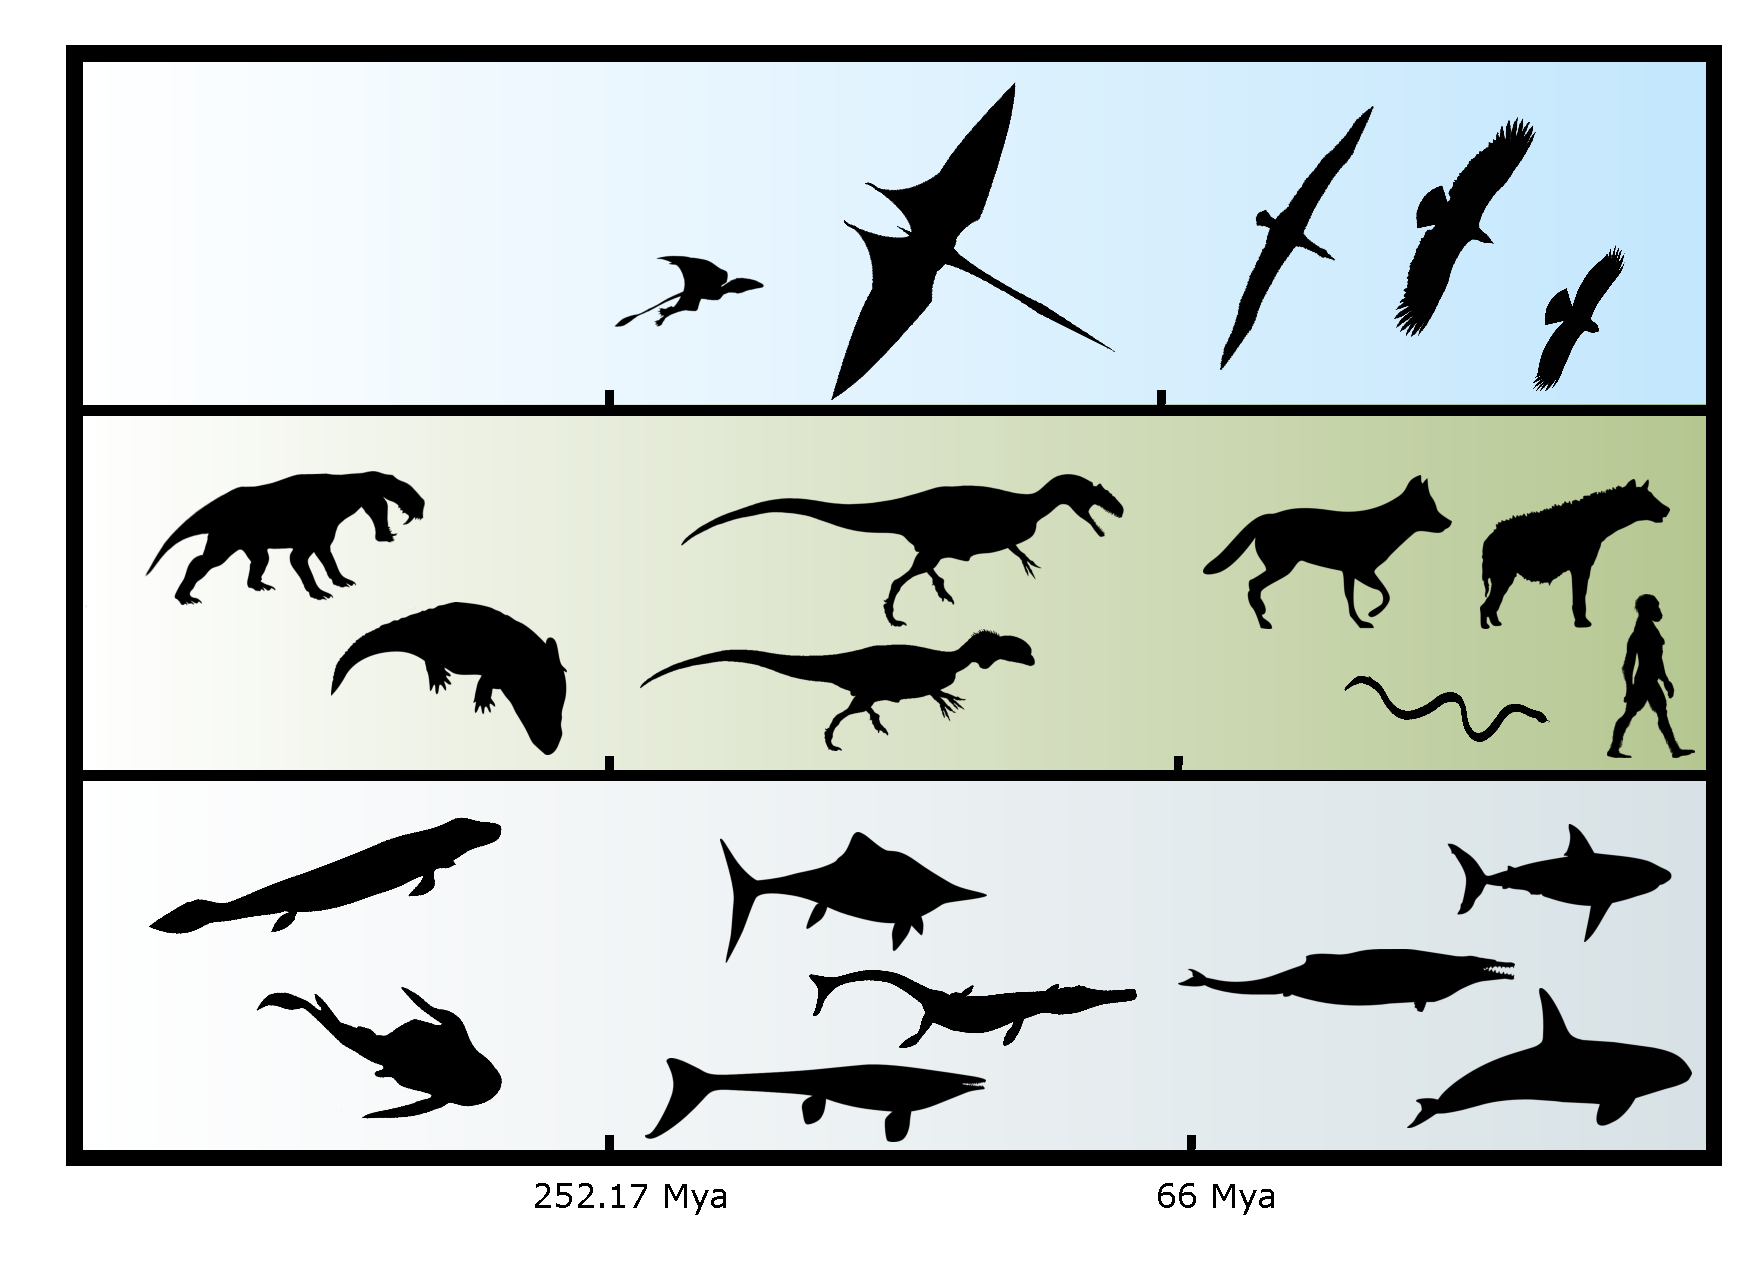
\includegraphics[width=1\textwidth]{timeline_figure/timeLine.pdf}
<<<<<<< HEAD
\caption{The diversity of scavengers through time across air, land and sea. Each species has either direct evidence for it being a scavenger or would be positioned high up on our scavenging scale. The ticks on the x axis represent the transitions for the Palaeozoic-Mesozoic (252.17 Mya) and Mesozoic-Cenozoic (66Mya) boundaries}
=======
\caption{The diversity of scavengers through time. Each species has either direct evidence for it being a scavenger or would be positioned high up on our scavenging scale. The three lines represent the three different environments (from top to bottom: aerial, terrestrial and aquatic). Time is represented on the horizontal axis with each third representing respectively the Paleozoic (541 to 252 Mya), the Mesozoic (252 to 66 Mya) and the Cenozoic (66 Mya to the present).}
%Silhouettes from left to right in each different environment: Aerial: \textit{Some pterosaur}, Azhdarchid (which one?), Diomedeidae, \textit{Gyps}, \textit{Some preybird}; Terrestrial: \textit{Some mammaliaform?}, \textit{Some temnospondyl?}, \textit{Allosaurus}?, \textit{Dilophosaurus}?, \textit{Canis lupus?}, \textit{Crocuta crocuta}, \textit{Some shneakyshnake}, \textit{Homo sapiens}; Aquatic: \textit{Tiktaalik}, \textit{Some antiarchplacoderm}, Ichtyosauridae, \textit{Some metriorhynchidae?}, Mosasauridae, \textit{Basilosaurus}, \textit{Carcharodon carcharias}, \textit{Orcinus orca}.
>>>>>>> origin/master
\label{Timeline}
\end{figure}


\section*{Conclusion} 
As is often the case in science, the present provides the key to the past.
The animals of today, while often different (sometimes radically so) to their ancestors, can be used to make informed comparisons to extinct species. 
We have used this technique to give insight into the drivers of scavenging across vertebrates through time.
In common with any other forager be they grazer, browser or predator, scavengers past and present have had to balance their energetic costs with the gains of food. 
The main factors we considered namely, encounter rate, handling time and prey availability can be used to create a scale of scavenging whereupon any species can be placed in order to establish the importance of carrion in it diet.
We hope this approach will be useful in the effort to explore this most understudied of feeding ecologies. 
% Add bits on climate change/dectection rate change, etc...

% KH Maybe we need to more strongly reaffirm that the framework that we give really is useful and should be applied to all sorts of things. etc

\section*{Appendix}
Scaling relationships for sustainable travel speed are 1.15 $\times$ body mass (kg) \textsuperscript{0.12} and 0.23 $\times$ body mass (kg) \textsuperscript{0.12} for mammals and reptiles respectively \citep{ruxton2004obligate}.
These are fed into the foraging model $\sfrac{\frac{\text{duration} \times \text{speed}}{2}}{1000}$ \citep{Enstipp2006Energetics}.

\section*{Acknowledgments}
Thanks to Natalie Cooper for highlighting the potential for this review, and to Ara Monadjem and Deirdre McClean for their comments on the manuscript. 

\newpage


\bibliography{bibfile}



\end{document}





%TG: what do you mean by their position? Phylogenetic? Position on the "scavenging scale"?


% This point illustrates how the environment can impact search efficiency depending on the sensory system that's used.






 


 


% \section*{Terrestrial Scavengers}

%\cite{ruxton2004obligate} offer a reason for this in that the traits that allow for vultures to exist as scavengers undermined their ability to hunt but that the same forces have not prevented mammals from doing so.


%\subsection*{Environment}




%TG: To be modified and inserted somewhere:

%TG: orginal sentence "The intertidal environment provides a ready food source of stranded marine animals on a twice-daily basis, in the immediate vicinity of the sea, and would thus have allowed marine ancestors of tetrapods gradually to acquire terrestrial competence while accessing a new and essentially untouched resource." 









 








% and sensory perception \citep{farlow1994speculations}.









 




%\section*{Aquatic Scavengers} 
%An aquatic environment presents challenges for direct observational studies and so, similar to the approaches involving extinct species, much work has approached the question of scavenging propensity from an energetics perspective.
%But it is certainly known to occur in many aquatic vertebrates.

%A point to note is that vertebrates are relatively rarer in aquatic environments, because even large animals can get support from the buoyancy of the water without needing a backbone.


%\subsection*{Locomotion}


%\subsection*{Detection}
%The existence of an obligate scavenger in a marine setting is uncertain \citep{britton1994marine,smith2003ecology,ruxton2004energetic,ruxton2005searching}.
%Depending on the species, a carcass in this environment either floats or descends to the sea floor \citep{Whitehead415}.
%In the latter low-light environment, visual detection distances are far lower (< 100 m) than they would be in the air.
%As such, animals detect resources through chemo- and mechanoreception more so than through vision \citep{ruxton2004energetic}. \cite{beasley2015vertebrates} do note that ``some benthic scavengers (e.g., hagfish: family Myxinidae) rely on necrophagy for a large portion of their diet and may indeed be obligate scavengers".




%\subsection*{Processing}


%\subsection*{Environment}

%Primary productivity is lower in almost all aquatic systems than terrestrial systems (except deserts) so as we go up the food chain the density of carcasses worth scavenging is going to be lower.










% Maybe drop this bit
% \section*{Ecological Role}
% It is recognised that scavengers keep energy flows at a higher trophic level in food webs than decomposers because they consume relatively more carrion \citep{devault2003scavenging}.
%They are also hugely important for the dispersal of nutrients \citep{beasley2015vertebrates}.
%Consider the diversity of animals that can end up feeding at the carcass of an elephant.
%Here we have an incredibly dense and nutrient rich patch that ends up being distributed widely.
%In the absence of vertebrate scavengers, invertebrates and microorganisms would consume the carcass in-situ or at least distribute the constituent nutrients over a much shorter range.
%This effect has been magnified as vertebrates evolved certain key traits that allowed them to range farther, namely an upright gait, an endothermic metabolism and of course, flight.
%To quantify this effect with a simple example we can turn to some allometric relationships relating sustainable travelling speed to body mass.
%In the case of mammals and reptiles these are 1.15 * body mass (kg) \textsuperscript{0.12} and 0.23 * body mass (kg) \textsuperscript{0.12}
% respectively \citep{ruxton2004obligate}.
%We can insert these into a foraging radius model ((duration * speed)/2)/1000 for a 12 hour foraging day which shows that while a 10 kg reptile can range 6.5 km an equally sized mammal can range nearly 33 km \citep{Enstipp2006Energetics}.
%Thus, in an ecological context, the evolution of these steps coupled with the ability to scavenge resulted in a world with a far more widely distributed nutrient landscape.





% %TG: LaTeX format template for the equations in the R file
% \begin{equation}
%   \text{Travelling speed} = \frac{duration \times speed}{2} \times 10^3
% \end{equation}
% where \textit{C} is a constant of $1.15$ for mammals and $0.23$ for squamates, %TG: if you meant squamates from reptiles
% and speed being:
% \begin{equation}
%   speed = C \times M^{0.12}
% \end{equation}


 
%Scavenging is a widespread behaviour among vertebrates where most if not all carnivores act as facultative scavengers.
%TG: or something more along the lines as:
%Most if not all carnivorous vertebrates are facultative scavenging behaviour to some extant.
%It is recognised that scavengers have an important role in keeping energy flows at a higher trophic level in food webs than decomposers because they consume relatively more carrion \citep{devault2003scavenging}. 
%Scavengers also provide useful ecosystem services by acting as barriers to the spread of disease by quickly consuming rotting carcasses which have often died from illness \citep{ogada2012dropping}.
%(Since we are intrested in scavanging in th paleo record ecosystem services might not be that relavent, although modulators of disease is still relavent) 





%The limitations in studying extant scavenging behaviour is much larger in extinct species and systems with the obvious lack of observational data available.
%TG: or more like this? 
% The limitations in studying scavenging in extant species are even bigger in extinct species and past systems since the obvious lack of available direct behavioural data (CITE) %TG: bet you there's some paper for that
% This means indirect observations in the fossil record and other approaches such as energetics must be used to infer these behaviours. %TG: I'll squiz your Am Nat paper here!
% One avenue to infer scavenging from palaeontological data can be achieved by determining if a prey item was simply too big for the carnivore to have tackled in cases where tooth marks are found \citep{pobiner2008paleoecological}. 
% Comparative analysis can also allow us to ascertain which morphologies and physiologies are likely to have been found in scavenging species in the past \citep{ruxton2004obligate}.
% The development of indirect measures of scavenging in palaeontology can in turn be applied to current scavenging systems that also suffer from a lack of observational data.

%§4
% In this review we collate methods (could this be another way of structuring it, just an idea) and research form palaeontology relating to scavenging behaviour and show that ignore this literature would be a missed opportunity for understanding extant scavenging.
%TG: totally agree. I think we need to clearly know what this review is about: scavenging through time (like a story line of scavenging past and present - a bit boring if I can speak my mind) or how to study scavenging (through time or any other aspect - probably more interesting to more people I guess).
%TG: additionally I find the divisions land/air/sea and Ceno/Meso/Paleozoic are a bit scholar. It might be better to just discuss the different techniques for investigating scavenging and include land/air/sea and Ceno/Meso/Paleo in there no? For example:
%\section{Method 1: direct observation}
%This can be totally doable in extant system for scavengers everywhere.
%It is advantageous because it's direct and reliable observations.
%But it has some limitations such as sending Adam to sit in the sun for ours and is hard to apply in deep sea environements or in any past ecosystems...



%remember the journal is an ecological one at heart so I would always keep in mind about making it useful for ecologists over paelo people. In particular from the website "ECOGRAPHY publishes papers focused on broad spatial and temporal patterns, particularly studies of population and community ecology, macroecology, biogeography, and ecological conservation. Studies in ecological genetics and historical ecology are welcomed in the context of explaining contemporary ecological patterns".



%"However, in general, vertebrate scavenging represents the widest dispersal of nutrients and energy from carcasses as vertebrate movement scales away to the broader landscape" \citep{benbow2015introduction}

 %"Increased kill rates by top predators may represent a little acknowledged marginal cost to the vertebrate community, directly attributable to scavenging activity. Given the impor -tance of top-down effects in many ecosystems, even a minor alteration to predation rates as driven by vertebrate scavengers may cause a significant flux in community composition."\citep{benbow2015introduction}

 %"Cortés-Avizanda et al. (2009) found that the abundance of prey species (i.e., hares—Lepus spp. and squirrels—Sciurus spp. in this case) decreased in sectors containing a carcass based on evidence from tracks in snow. An interesting hypothesis emerged, in which the scavengers that are recruited to a carcass may have temporarily played the dual role of increasing predator abundance near each carcass"\citep{benbow2015introduction}


%"Historically, the prevalence of scavenging activities has been greatly underestimated. However, upon recognition that (1) in most ecosystems, a large number of animals die from causes other than predation and thus become available to scavengers; (2) most carcasses are scavenged by vertebrates before they are completely decomposed by arthropods and bacteria; and (3) almost all carnivorous animals are facultative scavengers, the importance of scavenging in food webs seems unsurprising" \citep{benbow2015introduction}

%"This dispersion of carrion biomass by vertebrates is especially evident when carrion is initially concentrated spatially. For example, carcasses produced from fishing by-catch (Furness 2003), salmon (Salmonidae) die-offs (Hewson 1995), forest fires (Blanchard and Knight 1990), and single large carcasses (e.g., whales—Cetacea; Smith and Baco 2003) are often visited by multiple scavengers that range widely and therefore transport the nutrients from those carcasses over large distances."\citep{benbow2015introduction}

%"Cross-habitat nutrient transport can produce a variety of important outcomes in recipient systems (e.g., Polis et al. 2004), and scavengers can play a significant role in moving ``ecologi -cal subsidies" between habitats. For example, the use of ocean-derived carrion by terrestrial mammals (Rose and Polis 1998) and birds (Schlacher et al. 2013) is extensive and may strongly influence dynamics of coastal food webs."\citep{benbow2015introduction}

% "Markandya et al. (2008) estimated that the total costs to human health (including rabies cases from dog bites) that resulted from severe vulture declines totaled over $34 billion from 1993 to 2006. Also, Ogada et al. (2012) determined that the exclusion of vultures from large animal carcasses in Kenya resulted in a tripling of carcass decomposition times."\citep{benbow2015introduction}

%"Of all the mammalian carnivores in Africa, brown, striped, and spotted hyenas (hereafter referred to simply as hyenas) derive the largest portion of their diet from scavenging. This is not surprising, as they show many unique adaptations specifically for scavenging. They have a unique body posture and a ``rocking-horse" gait (Eloff 1964; Tilson and Henschel 1986; Hofer and East 1993a; Frank 1996) that allows them to cover long distances in search of carrion and prey."\citep{benbow2015introduction}



%\textit{Allosaurus} tooth marks on a hadrosaur in the Late Jurassic. 
% Late Triassic scavenging on a prosauropod by basal carnivorous archosaurs \citep{hungerbuhler1998taphonomy}.
%A likely instance of scavenging between a 4-million-year-old white shark (\textit{Carcharodon}) and mysticete whale from Peru \citep{ehret2009caught}.
%Bite marks on early Holocene Tursiops truncatus fossils from the North Sea indicate scavenging by rays (Chondrichthyes, Rajidae) \citep{van2009bite}. 
%Possible scavenging on a juvenile fur seal from the Late Neogene \citep{boessenecker2011mammalian}. 







